\chapter{Network Embedding}


\section{Introduction}
\begin{itemize}
    \item Graph embedding aims to \textbf{map each node in a given graph into a low-dimensional vector representation} that typically preserves some key information of the node in the original graph.
    \item A node in a graph can be viewed from two domains:
    \begin{itemize}
        \item The original graph domain, where nodes are connected via edges
        \item The embedding domain, where each node is represented as a continuous vector.
    \end{itemize}
    \item Using this embedding we can perform graph clustering, classification using the machine learning algorithms.
    \begin{figure}[h] 
        \centering
        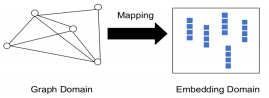
\includegraphics[height=3cm, width=7cm]{tex/img/Embedding.png} 
    \end{figure}
\end{itemize}
\section{Algorithms}
    Algorithms for finding these embedding
    \begin{itemize}
        \item DeepWalk
        \item Node2Vec
    \end{itemize}
\newpage
\section{Deepwalk}
\paragraph{}\textbf{DeepWalk} is a supervised learning algorithm developed to analyze graphs for classification, clustering, similarity search, and representations for statistical models.
\subsection{Step1}
    \paragraph{} Generate a set of random walks of size $\mathcal{T}$.
\subsubsection{Random Walk}
    \paragraph{}Let $\mathcal{G}$=\{ $\mathcal{V}$,$\mathcal{E}$ \} be a graph. We consider a random walk starting from the node $v^{(t)}$ $\epsilon$ $\mathcal{V}$. 
    The probability of choosing a next node is given by.
    \begin{equation}
        p(v^{(t+1)}|v^{(t)}) = \frac{1}{d(v^{(t)})}, v ^{(t+1)} \epsilon \ \mathcal{N}(v^{(t)}) \\
    \end{equation}
    \begin{equation}
        p(v^{(t+1)}|v^{(t)}) = 0 \ \ otherwise
    \end{equation}
    \paragraph{} Example of random walk with length 2
    \begin{figure}[h]
        \centering
        \begin{subfigure}[b]{0.5\textwidth}
                    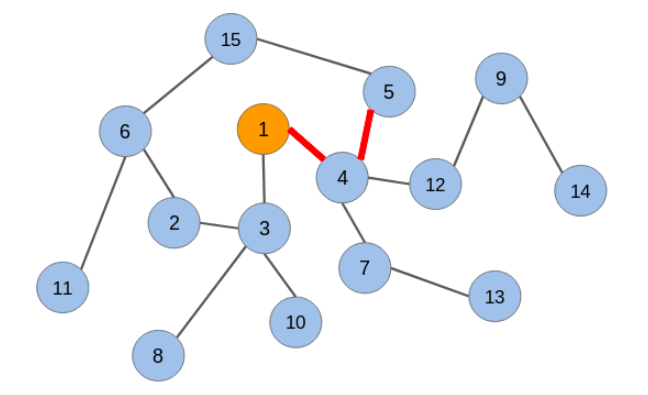
\includegraphics[width=\textwidth]{tex/img/G1.png}
                    \caption{random walk 1}
            \end{subfigure}%
            \hfill
        \begin{subfigure}[b]{0.5\textwidth}
                    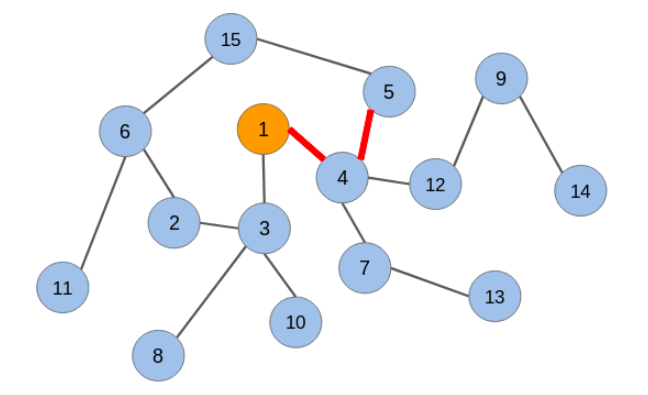
\includegraphics[width=\textwidth]{tex/img/G1.png}
                    \caption{random walk 2}
           \end{subfigure}%
        \end{figure}
    \subsection{Step2}
\paragraph{} Considering the set of random walk as set of vocabulary for which \textbf{Skip gram} model can be used to find the node embedding.
\subsubsection{Skip gram model}
\paragraph{} Skim gram is algorithm in language modeling tries to preserve the information of the sentences by capturing the \textbf{co-occurrence relations between words in these sentences}.


    